\documentclass[11pt]{amsart}
\usepackage{color,amssymb,amsthm,amstext,latexsym,amsmath,amscd,amsfonts}
\usepackage{tikz}
\usepackage{tcolorbox}
\usepackage{tikz}
\usepackage{tikz-cd}
\usetikzlibrary{calc}

\begin{document}

  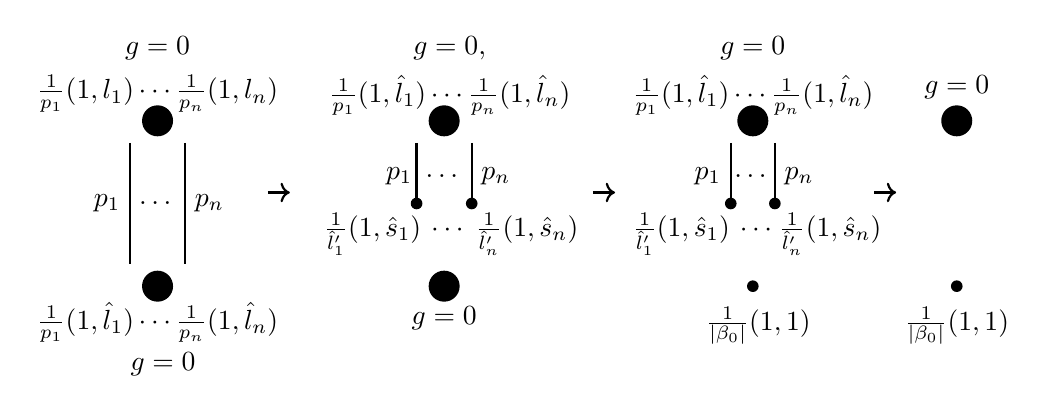
\begin{tikzpicture}[scale=.7]	
    \coordinate (point) at  (-0.5,3);
    \fill  (5.5,4) circle (8pt);
    \fill  (5.5,1) circle (8pt);
    \coordinate[label=above:{$\frac{1}{p_1}(1,\hat{l}_1) \cdots \frac{1}{p_n}(1,\hat{l}_n)$}] (VFD) at (5.5,-.2);
    \coordinate[label=above:{$g=0$}] (VFE) at (5.6,-0.8);			
    \coordinate[label=below:{$\frac{1}{p_1}(1,l_1)\cdots \frac{1}{p_n}(1,l_n)$}] (VCC) at (5.5,5);
    \coordinate[label=below:{$g=0$}] (VCC) at (5.5,5.7);			
    \draw[thick](5,3.6) -- (5,1.4);
    \draw[thick](6,3.6) -- (6,1.4);
    \node at ($(5,2.5)!.5!(6,2.5)$) {\ldots};
    \coordinate[label=right:{$p_n$}] (c1) at (6,2.5);
    \coordinate[label=left:{$p_1$}] (c1) at (5,2.5);		

    %%%%%%%%%%%%%%%%%%%%%%%%%%
    \draw[->, thick] (7.5,2.7) to (7.9,2.7);	
    %%%%%%%%%%%%%%%%%%%%%%%%%%

    \fill  (10.7,4) circle (8pt);
    \fill  (10.2,2.5) circle (3pt);
    \fill  (11.2,2.5) circle (3pt);
    \fill  (10.7,1) circle (8pt);
\coordinate[label=below:{$g=0$}] (VFE) at (10.7,.8);		
\coordinate[label=below:{$g=0,$}] (VCC) at (10.8,5.7);	
\coordinate[label=below:{$\frac{1}{p_1}(1,\hat{l}_1) \cdots \frac{1}{p_n}(1,\hat{l}_n)$}] (VCC) at (10.8,5);
\coordinate[label=below:{$\frac{1}{\hat{l}_1^\prime}(1,\hat{s}_1)$}] (VCC) at (9.4,2.5);
\coordinate[label=below:{$\cdots$}] (VCC) at (10.8,2.3);
\coordinate[label=below:{$\frac{1}{\hat{l}_n^\prime}(1,\hat{s}_n)$}] (VCC) at (12.2,2.5);

\draw[thick](10.2,3.6) -- (10.2,2.5);
\node at ($(10.2,3)!.5!(11.2,3)$) {\ldots};
\draw[thick](11.2,3.6) -- (11.2,2.5);

\coordinate[label=right:{$p_n$}] (c1) at (11.2,3);
\coordinate[label=left:{$p_1$}] (c1) at (10.3,3);	

%%%%%%%%%%%%%%%%%%%%%%%%%%
 \draw[->, thick] (13.4,2.7) to (13.8,2.7);	
 %%%%%%%%%%%%%%%%%%%%%%%%%%

\fill  (16.3,4) circle (8pt);
\fill  (15.9,2.5) circle (3pt);
\fill  (16.7,2.5) circle (3pt);
\fill  (16.3,1) circle (3pt);

\coordinate[label=below:{$\frac{1}{\lvert \beta_0\rvert }(1,1)$}] (VFE) at (16.4,.8);		
\coordinate[label=below:{$g=0$}] (VCC) at (16.3,5.7);	
\coordinate[label=below:{$\frac{1}{p_1}(1,\hat{l}_1) \cdots \frac{1}{p_n}(1,\hat{l}_n)$}] (VCC) at (16.3,5);
\coordinate[label=below:{$\frac{1}{\hat{l}_1^\prime}(1,\hat{s}_1)$}] (VCC) at (15,2.5);
\coordinate[label=below:{$\cdots$}] (VCC) at (16.4,2.3);
\coordinate[label=below:{$\frac{1}{\hat{l}_n^\prime}(1,\hat{s}_n)$}] (VCC) at (17.7,2.5);

\draw[thick](15.9,3.6) -- (15.9,2.5);
\node at ($(15.9,3)!.5!(16.7,3)$) {\ldots};
\draw[thick](16.7,3.6) -- (16.7,2.5);

\coordinate[label=right:{$p_n$}] (c1) at (16.7,3);
\coordinate[label=left:{$p_1$}] (c1) at (15.9,3);	

%%%%%%%%%%%%%%%%%%%%%%%%%
 \draw[->, thick] (18.5,2.7) to (18.9,2.7);	
%%%%%%%%%%%%%%%%%%%%%%%%%%

\fill  (20,4) circle (8pt);
\fill  (20,1) circle (3pt);

\coordinate[label=below:{$\frac{1}{\lvert \beta_0\rvert }(1,1)$}] (VFE) at (20,.8);	
\coordinate[label=below:{$g=0$}] (VCC) at (20,5);	

\end{tikzpicture}

\end{document}